\documentclass[a4paper]{article}

%%%%%%%%%%%%%%%%
%%% PREAMBLE %%%
%%%%%%%%%%%%%%%%

%%% PACKAGES %%%
\usepackage{fontspec}                     % set fonts
	\setmainfont{Junicode}
\usepackage[a4paper,margin=3cm]{geometry} % page layout
\usepackage[svgnames]{xcolor}             % rainbowssss *_*
\usepackage{hyperref}                     % enhanced references (links)
	\hypersetup{%
		colorlinks=true,
		allcolors=NavyBlue}
\usepackage{fancyhdr}                     % headers & footers
\usepackage{titling}                      % macros \thetitle, \theauthor
\usepackage{graphicx}                     % enhanced graphics support
	\graphicspath{{img/}}
\usepackage[toc]{glossaries}              % glossaries (obv)
	\setglossarystyle{altlisthypergroup}
	\makeglossaries
	\newglossaryentry{turnstile}
{%
	name=turnstile,
	description={An ingress control device to help with the organizization
	of the passengers’ boarding. Basically a lockable revolving gate with
	three arms. When signalled, the gate unlocks and a single passenger may
	go through by turning one of the arms. After a single rotation, the gate
	locks again, waiting for the next signal.}
}

\newglossaryentry{authentication}
{%
	name=authentication,
	description={The process of verifying the \textit{identity} of the
	passengers.}
}

\newglossaryentry{authorization}
{%
	name=authorization,
	description={The process of veryfying whether an identified passenger
	has \textit{permission} to do something (eg board the bus).}
}

\newglossaryentry{alarm}
{%
	name=alarm,
	description={A device installed at every door that emits light and sound
	to draw attention to certain events. For instance, it signals the end of
	the boarding phase and also turns on in the event of an unauthorized
	boarding attempt.}
}

\newglossaryentry{RFIDScanner}
{%
	name={RFID scanner},
	description={An instrument capable of reading radio frequency
	identification tags. This can be used to effectively identify
	passengers.}
}

\newglossaryentry{boardingController}
{%
	name={boarding controller},
	description={A device responsible for the orchestration of the whole
	boarding phase (signalling doors to open or close, activating the alarm,
	etc).}
}

\usepackage{tabularx}                     % enhanced tables
\usepackage[noabbrev]{cleveref}           % clever references
\usepackage{booktabs}                     % pretty tables
\usepackage{xfrac}                        % pretty fractions
\usepackage{interval}                     % well, intervals
\usepackage{siunitx}                      % SI units
	\sisetup{per-mode=fraction,fraction-function=\sfrac}

%%% OTHER %%%
\setlength\headheight{22.62152pt}

%%% META %%%
\title{Assignment \#4 \\ Safety Analysis}
\author{Levendula}
\date{\today}

%%% ADDITIONAL PACKAGE CONFIG %%%
% fancyhdr
\pagestyle{fancy}
\fancyhf{}
\lhead{\theauthor}
\rhead{\thetitle}
\lfoot{\today}
\rfoot{\thepage}

%%%%%%%%%%%%%%%%%%%%%%%%%%%%%%%%%%%%%%%%%%%%%%%%%%%%%%%%%%%%%%%%%%%%%%%%%%%%%%%%

%%%%%%%%%%%%
%%% BODY %%%
%%%%%%%%%%%%

\begin{document}

\begin{titlepage}
	\begin{center}
		
\includegraphics[width=8cm]{logo.jpg}

		\vspace{.2cm}

		\textbf{Budapest University of Technology and Economics} \\
		Faculty of Electrical Engineering and Informatics \\
		Department of Measurement and Information Systems \\

		\vspace{2cm}

		{\huge IT System Design (\texttt{VIMIAC01})}

		\vspace{2cm}

		{\huge \bfseries \thetitle}

		\vspace{.5cm}

		{\Large \theauthor}

		\vspace{.5cm}

		{\Large \today}
	\end{center}

	\vfill{}

	{\large Team members:}

	\vspace{.25cm}

	\begin{tabular}{lll}
		Annamária Gálik &
			\texttt{WGMUO2} &
			ancsi666@gmail.com \\
		Borbála Szilágyi &
			\texttt{COVQ1M} &
			szilagyiborbala8@gmail.com \\
		Bertalan Z. Péter &
			\texttt{QO7CU6} &
			bertalan.peter+uni@bertalanp99.eu
	\end{tabular}

	\vspace{2cm}
\end{titlepage}


\tableofcontents
\listoffigures
\listoftables
\clearpage



% ------------------------------------------------------------------------------
\section{Our task}

We were assigned with the safety analysis of the \gls{ACC} component,
specifically the \gls{wheelSpeedSensor} component, which is capable of measuring
the vehicle's speed. Since the speed sensor by itself isn't especially reliable,
there is also a \gls{selfCheck} mechanism in the system.

In the first iteration, we calculated the reliability of the \gls{ACC} component
based on the unrelability values of the components. We also determined how
detrminental to reliability using a cheaper microcontroller for the system would
be.

In the second iteration, we analysed the effects of adding a second
\gls{wheelSpeedSensor} (later even an additional third one) to the system.



% ------------------------------------------------------------------------------
\section{Solutions}


% - - - - - - - - - - - - - - - - - - - - - - - - - - - - - - - - - - - - - - -
\subsection{First iteration}

% -  -  -  -  -  -  -  -  -  -  -  -  -  -  -  -  -  -  -  -  -  -  -  -  -  -
\subsubsection{Failure modes for the self check component}\label{ssub:failmodes}

\begin{enumerate}
	\item Implausible speed data received

		\textbf{Self-check}: make sure speed data is within reasonable
		range

		Every time a new speed value is received, a check should be
		performed that the value is within a predefined range (eg
		\(\interval{0}{\SI{150}{\km\per\hour}}\)). If not
		(negative or extremely high), it should be discarded. There
		should be margin for error, but if this happens consistently,
		the system is too dangerous to use and should be shut down.

	\item Absurd measurement deltas

		\textbf{Self-check}: keep track of deltas and make sure they
		don't exceed reasonable values

		Keeping the last received value in memory for each new
		reception, if the next data arrived in time and the difference
		is absurdly large, there must be some failure in the system (eg
		the vehicle could not have accelerated from 10
		\(\si{\km\per\hour}\) to 140 in 5 milliseconds). As with
		the previous failure mode, perhaps this can be tolerated at
		times, but normally, it also indicates serious malfunction.

	\item Interval between measurements too large

		\textbf{Self-check}: measure time from last received data until
		next

		This basically the same failure mode that was already given to
		us in the assignment description, phrased differently.
		Obviously, the system cannot be used safely if speed data isn't
		received regularly with acceptably little intervals of time
		between receptions. If this interval exceeds a predefined amount
		of time, the system should be deemed too dangerous to trust.
\end{enumerate}

% -  -  -  -  -  -  -  -  -  -  -  -  -  -  -  -  -  -  -  -  -  -  -  -  -  -
\subsubsection{Fault tree belonging to ‘The ACC does not apply the brakes when
               the vehicle is moving too fast’}

Although our solution can be found in the TopEvent FTA project file, we have
also added a screenshot of the tree which can be seen on
\cref{fig:fault_tree_original}.

\begin{figure}
	\centering
	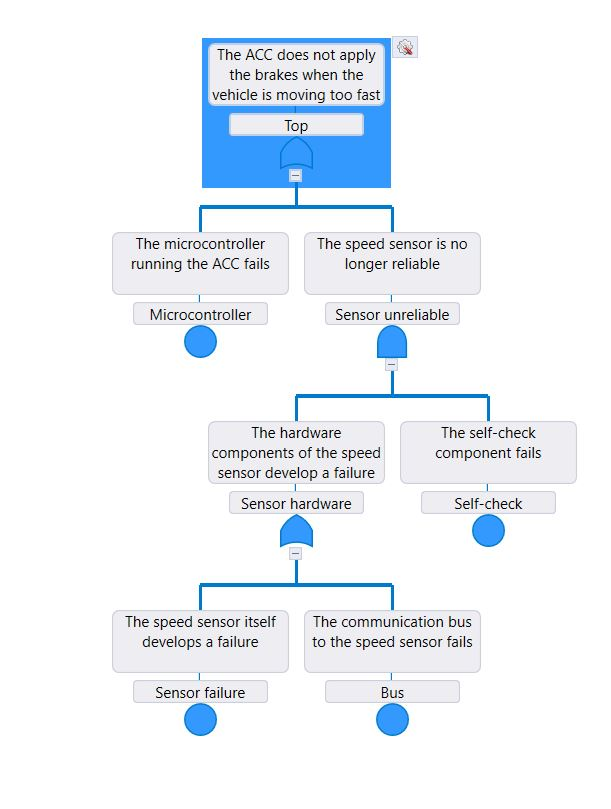
\includegraphics[width=.5\textwidth]{fault_tree_original.jpg}
	\caption{Fault tree of the requested top level hazard}%
	\label{fig:fault_tree_original}
\end{figure}

% -  -  -  -  -  -  -  -  -  -  -  -  -  -  -  -  -  -  -  -  -  -  -  -  -  -
\subsubsection{Single Point(s) of Failure}

It can be seen from the model that the only \gls{SPOF} is the
\emph{microcontroller}. All other events can happen (by themselves) and the
hazard should still not occur.

% -  -  -  -  -  -  -  -  -  -  -  -  -  -  -  -  -  -  -  -  -  -  -  -  -  -
\pagebreak
\subsubsection{Unavailablity of top level event}

The complete list of the unavailability values we have used can be seen on
\cref{tab:unreliability_original}. Italics indicate values that we invented
ourselves because they weren't given. Using these, the program evaluated the
following unrealiability value for the top-level event:

\[ Q = 0.00506 \]

(this can be seen on \cref{fig:eval_original})

\begin{table}
	\centering
	\begin{tabular}{ll}
		\toprule
		microcontroller          & \(0.005\) \\
		\gls{wheelSpeedSensor}   & \(0.01\)  \\
		communication bus        & \(0.002\) \\
		\textit{\gls{selfCheck}} & \(0.005\) \\
		\bottomrule
	\end{tabular}
	\caption{Table of unreliability values for the first iteration}%
	\label{tab:unreliability_original}
\end{table}

This value can be confirmed by manual calculation: starting from bottom to top,
values for each \emph{or} gate are to be added together. For \emph{and} gates,
we must mutliply them (these are just some basic priciples of probability
theory). Therefore

\[ Q = \left((0.01 + 0.002) \times 0.005\right) + 0.005 = 0.00506 \]

\begin{figure}
	\centering
	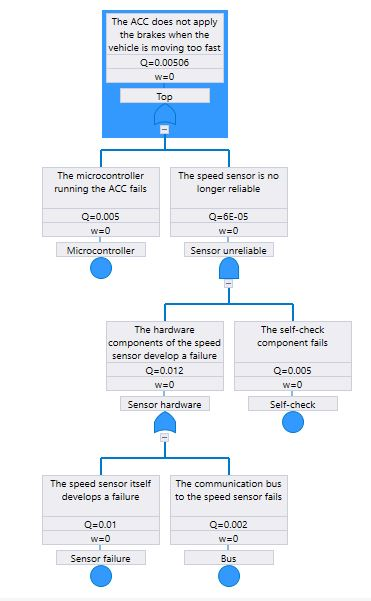
\includegraphics[width=.5\textwidth]{eval_original.jpg}
	\caption{Evaluation of the top level hazard}%
	\label{fig:eval_original}
\end{figure}

% -  -  -  -  -  -  -  -  -  -  -  -  -  -  -  -  -  -  -  -  -  -  -  -  -  -
\subsubsection{Using a cheaper microcontroller}

The cheaper microcontroller cuts back on reliability as well as costs. In fact,
it is half as reliable as the original, thus we set it's unreability value to
\(0.01\).

Now the evaluation goes as seen on \cref{fig:eval_cheap}. Manually:

\[ Q = \left((0.01 + 0.002) \times 0.005\right) + 0.01 = 0.01006 \]

\begin{figure}
	\centering
	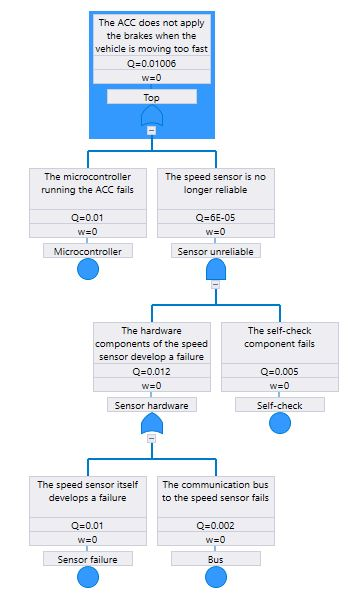
\includegraphics[width=.47\textwidth]{eval_cheap.jpg}
	\caption{Evaluation of the top level hazard with cheaper
	         microcontroller}%
	\label{fig:eval_cheap}
\end{figure}


% - - - - - - - - - - - - - - - - - - - - - - - - - - - - - - - - - - - - - - -
\subsection{Second iteration}

% -  -  -  -  -  -  -  -  -  -  -  -  -  -  -  -  -  -  -  -  -  -  -  -  -  -
\subsubsection{Behaviour of the comparison logic}

Now that there are two sensors, the error tolerance is slightly increased. For
every failure mode mentioned in \cref{ssub:failmodes}, the other sensor's data
can also be taken into consideration. If the other sensor provides meaningful
data, then that should be used and the other sensor's data should be discarded.
However, it may also be possible that both sensors send acceptable, but
inconsistent data: in this case, we decided it's best to use the data which is
more ‘critical’; eg out of two speed values that aren't equal, it is better to
use the higher one, as the consequences of that being wrong and braking
unnecessariliy are less dangerous than being unaware of overly high speeds.

% -  -  -  -  -  -  -  -  -  -  -  -  -  -  -  -  -  -  -  -  -  -  -  -  -  -
\subsubsection{Extending the fault tree}

The extended fault tree can be seen on \cref{fig:fault_tree_extended}. In
addition to the original, it contains another \gls{wheelSpeedSensor} branch and
also the comparator component.

We have evaluated the tree with the unrealibility values seen on
\cref{tab:unreliability_extended} (again, italics indicate improvised values).

\begin{table}
	\centering
	\begin{tabular}{ll}
		\toprule
		microcontroller          & \(0.005\) \\
		\gls{wheelSpeedSensor}   & \(0.01\)  \\
		communication bus        & \(0.002\) \\
		\textit{\gls{selfCheck}} & \(0.005\) \\
		\textit{comparator}      & \(0.001\) \\
		\bottomrule
	\end{tabular}
	\caption{Table of unreliability values for the second iteration}%
	\label{tab:unreliability_extended}
\end{table}

Now, as seen on \cref{fig:eval_extended}, the unreliability value of the
top-level hazard is:

\[ Q = {\left((0.01 + 0.002) \times 0.005\right)}^2 + 0.005 + 0.001 = 0.006 \]

\begin{figure}
	\centering
	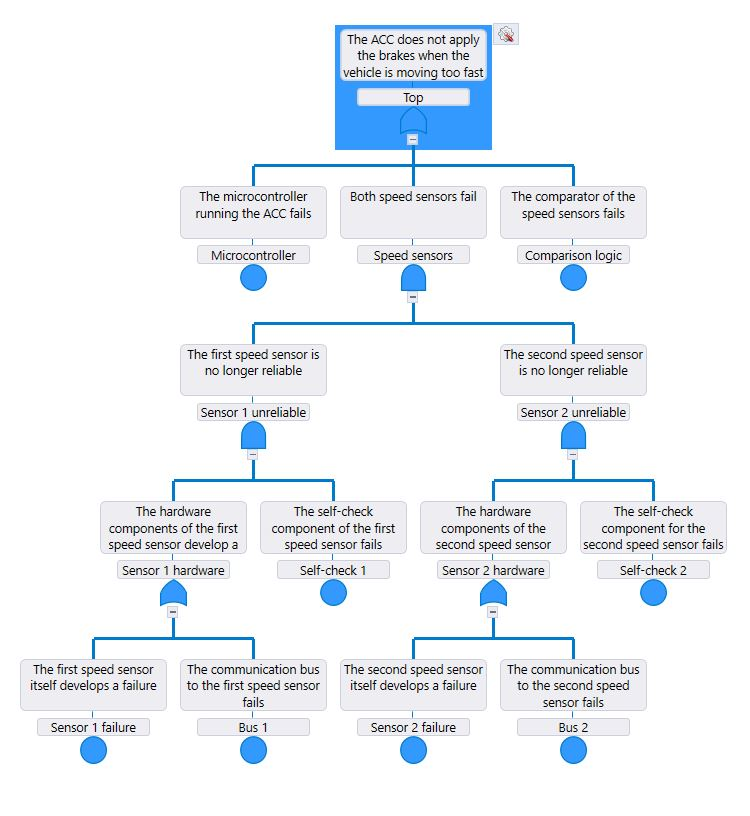
\includegraphics[width=.5\textwidth]{fault_tree_extended.jpg}
	\caption{Fault tree extended with the second sensor}%
	\label{fig:fault_tree_extended}
\end{figure}

\begin{figure}
	\centering
	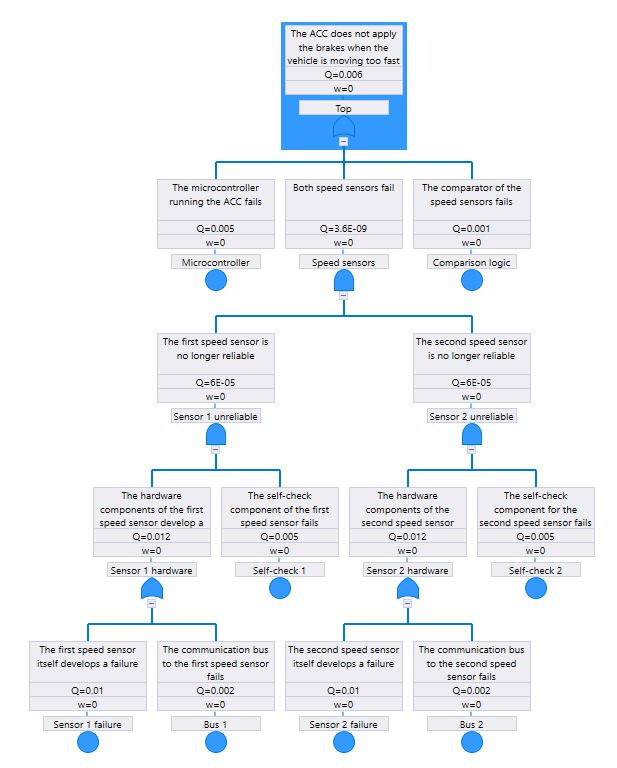
\includegraphics[width=.5\textwidth]{eval_extended.jpg}
	\caption{Evaluation of the top level hazard with the two speed sensors}%
	\label{fig:eval_extended}
\end{figure}


% -  -  -  -  -  -  -  -  -  -  -  -  -  -  -  -  -  -  -  -  -  -  -  -  -  -
\subsubsection{Adding a third sensor}

Seeing what little improvement adding a second sensor had, it is highly unlikely
a third one would matter much. Nevertheless, we added another branch and
reevaluated te model to see. The last fault tree can be seen on
\cref{fig:fault_tree_imsc} and the calculation of the unreability values on
\cref{fig:eval_imsc}.

According to the software used, the diffence is so insignificant, it does not
even show:

\[ Q = 0.006 \]

Calculating manually we found how minute the differece is:

\[
	\begin{aligned}
		Q_2 &= {\left((0.01 + 0.002) \times 0.005\right)}^2
		       + 0.005 + 0.001
		     = 0.006000003 \\
		Q_3 &= {\left((0.01 + 0.002) \times 0.005\right)}^3
		       + 0.005 + 0.001
		     = 0.006000000 \\
		& \Downarrow \\
		\Delta Q &= 3.6 \times 10^{-9}
	\end{aligned}
\]

With three sensors, the comparator component should implement a voting
mechanism, for the three sensors.

\begin{figure}
	\centering
	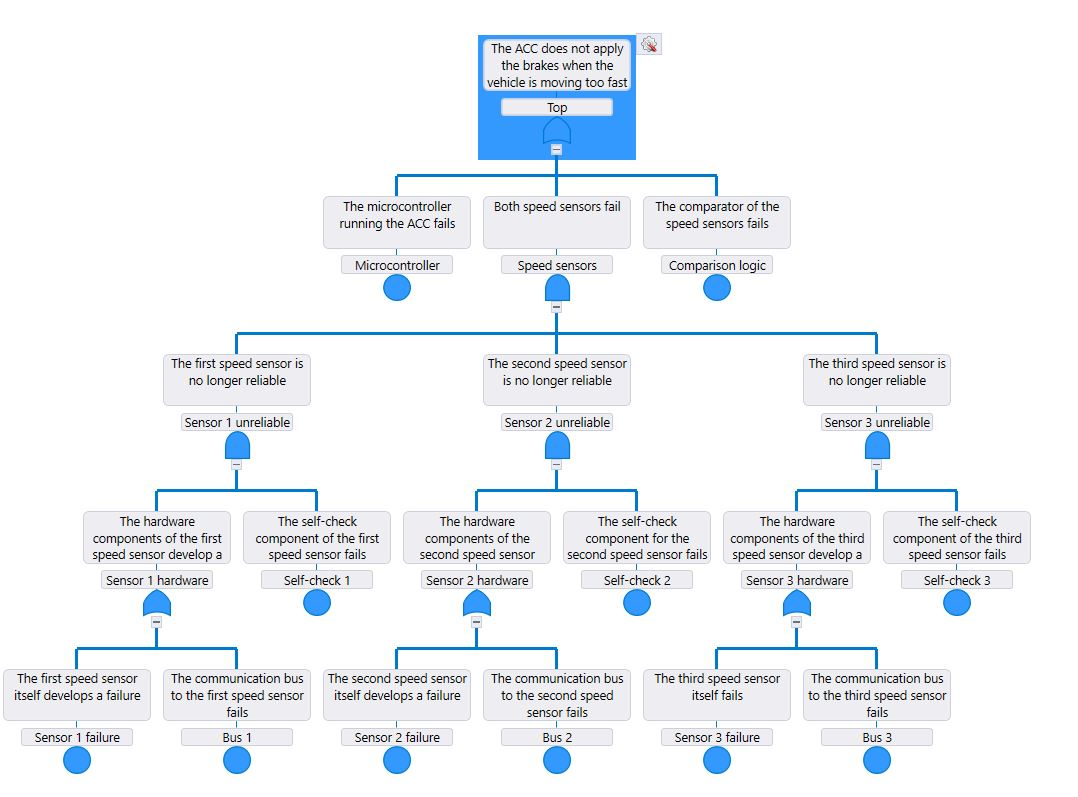
\includegraphics[width=\textwidth]{fault_tree_imsc.jpg}
	\caption{Fault tree with three speed sensors}%
	\label{fig:fault_tree_imsc}
\end{figure}

\begin{figure}
	\centering
	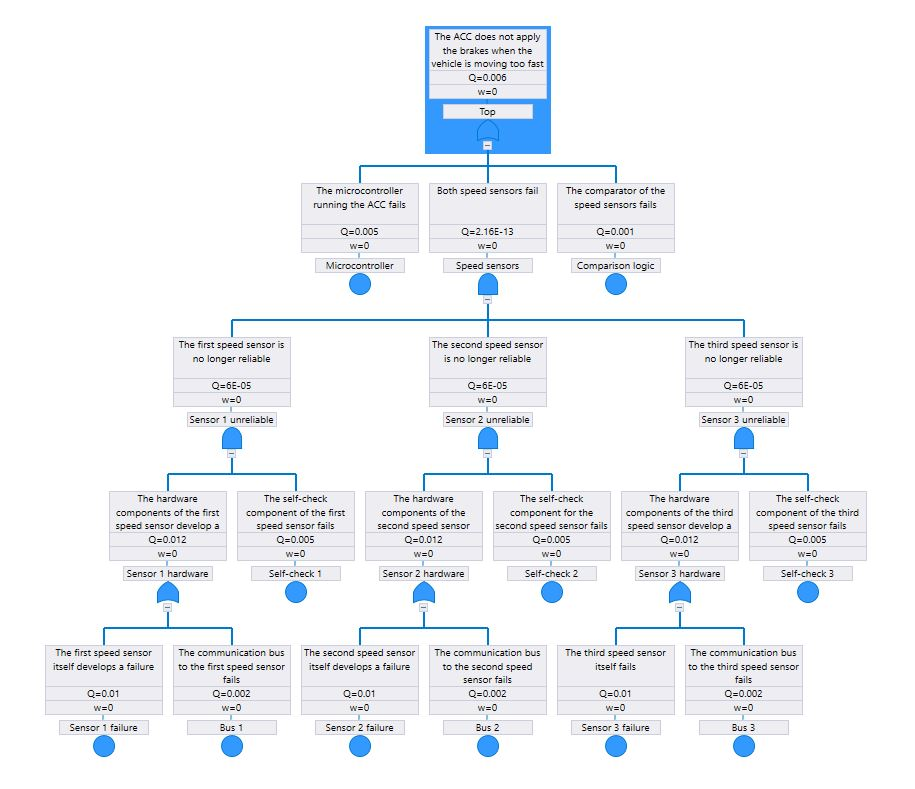
\includegraphics[width=\textwidth]{eval_imsc.jpg}
	\caption{Evaluation of the top level hazard with three speed sensors}%
	\label{fig:eval_imsc}
\end{figure}



% ------------------------------------------------------------------------------
\section{Work journal}

\begin{tabularx}{\textwidth}{l l l X}
	\toprule
	Team member & Date & Time\footnote{in hours} & Activity \\ \midrule

	Borbála Szilágyi  & 2019-11-16 & 1.5 & 1st iteration: ideas         \\
	Annamária Gálik   & 2019-11-16 & 1.5 & 1st iteration: ideas         \\
	Bertalan Z. Péter & 2019-11-16 & 1   & 1st iteration: diagrams      \\
	Borbála Szilágyi  & 2019-11-17 & 0.5 & 2nd iteration: ideas         \\
	Annamária Gálik   & 2019-11-17 & 0.5 & 2nd iteration: ideas         \\
	Bertalan Z. Péter & 2019-11-17 & 0.5 & 2nd iteration: diagrams      \\
	Borbála Szilágyi  & 2019-11-17 & 0.5 & checking the completed tasks \\
	Bertalan Z. Péter & 2019-11-18 & 0.5 & documentation                \\
	\bottomrule
\end{tabularx}

\clearpage
\printglossaries

\end{document}
